\documentclass[
a4paper,     %% defines the paper size: a4paper (default), a5paper, letterpaper, ...
% landscape,   %% sets the orientation to landscape
% twoside,     %% changes to a two-page-layout (alternatively: oneside)
% twocolumn,   %% changes to a two-column-layout
% headsepline, %% add a horizontal line below the column title
% footsepline, %% add a horizontal line above the page footer
% titlepage,   %% only the titlepage (using titlepage-environment) appears on the first page (alternatively: notitlepage)
% parskip,     %% insert an empty line between two paragraphs (alternatively: halfparskip, ...)
% leqno,       %% equation numbers left (instead of right)
% fleqn,       %% equation left-justified (instead of centered)
% tablecaptionabove, %% captions of tables are above the tables (alternatively: tablecaptionbelow)
% draft,       %% produce only a draft version (mark lines that need manual edition and don't show graphics)
% 10pt         %% set default font size to 10 point
% 11pt         %% set default font size to 11 point
11pt         %% set default font size to 12 point
]{scrartcl}  %% article, see KOMA documentation (scrguide.dvi)


 %%% File-Information {{{
%%% Filename: template_bericht.tex
%%% Purpose: lab report, technical report, project report
%%% Time-stamp: <2004-06-30 18:19:32 mp>
%%% Authors: The LaTeX@TUG-Team [http://latex.tugraz.at/]:
%%%          Karl Voit (vk), Michael Prokop (mp), Stefan Sollerer (ss)
%%% History:
%%%   20050914 (ss) correction of "backref=true" to "backref" due to hyperref documentation
%%%   20040630 (mp) added comments to foldmethod at end of file
%%%   20040625 (vk,ss) initial version
%%%
%%% Notes:
%%%
%%%
%%%
%%% }}}


%%%%%%%%%%%%%%%%%%%%%%%%%%%%%%%%%%%%%%%%%%%%%%%%%%%%%%%%%%%%%%%%%%%%%%%%%%%%%%%%
%%%
%%% packages
%%%


\usepackage[a4paper]{geometry}
\geometry{tmargin=1in,bmargin=1.25in,lmargin=2.5cm,rmargin=2cm}

\usepackage{microtype}

%%%
%%% encoding and language set
%%%

%%% ngerman: language set to new-german
\usepackage[english]{babel} 
\usepackage{tocloft}
\usepackage{subcaption}
\usepackage{listings}
\usepackage{color} %red, green, blue, yellow, cyan, magenta, black, white
\usepackage{courier}
\usepackage{float}

\usepackage{siunitx}

%%% babel: language set (can cause some conflicts with package ngerman)
%%%        use it only for multi-language documents or non-german ones
%\usepackage[ngerman]{babel}

%%% inputenc: coding of german special characters
\usepackage[latin1]{inputenc}

%%% fontenc, ae, aecompl: coding of characters in PDF documents
\usepackage[T1]{fontenc}
\usepackage{ae,aecompl}

%%%
%%% technical packages
%%%

%%% amsmath, amssymb, amstext: support for mathematics
%\usepackage{amsmath,amssymb,amstext}

\usepackage{bm}

%%% psfrag: replace PostScript fonts
\usepackage{psfrag}

%%% listings: include programming code
%\usepackage{listings}

%%% units: technical units
%\usepackage{units}

%%%
%%% layout
%%%

%%% scrpage2: KOMA heading and footer
%%% Note: if you don't use this package, please remove 
%%%       \pagestyle{scrheadings} and corresponding settings
%%%       below too.
\usepackage[automark]{scrpage2}


%%%
%%% PDF
%%%

\usepackage{ifpdf}

%%% Should be LAST usepackage-call!
%%% For docu on that, see reference on package ``hyperref''
\ifpdf%   (definitions for using pdflatex instead of latex)

  %%% graphicx: support for graphics
  \usepackage[pdftex]{graphicx}

  \pdfcompresslevel=9

  %%% hyperref (hyperlinks in PDF): for more options or more detailed
  %%%          explanations, see the documentation of the hyperref-package
  \usepackage[%
    %%% general options
    %pdftex=true,      %% sets up hyperref for use with the pdftex program
    %plainpages=false, %% set it to false, if pdflatex complains: ``destination with same identifier already exists''
    %
    %%% extension options
    backref,      %% adds a backlink text to the end of each item in the bibliography
    pagebackref=false, %% if true, creates backward references as a list of page numbers in the bibliography
    colorlinks=false,   %% turn on colored links (true is better for on-screen reading, false is better for printout versions)
    %
    %%% PDF-specific display options
    bookmarks=true,          %% if true, generate PDF bookmarks (requires two passes of pdflatex)
    bookmarksopen=false,     %% if true, show all PDF bookmarks expanded
    bookmarksnumbered=false, %% if true, add the section numbers to the bookmarks
    %pdfstartpage={1},        %% determines, on which page the PDF file is opened
    pdfpagemode=UseNone         %% None, UseOutlines (=show bookmarks), UseThumbs (show thumbnails), FullScreen
  ]{hyperref}


  %%% provide all graphics (also) in this format, so you don't have
  %%% to add the file extensions to the \includegraphics-command
  %%% and/or you don't have to distinguish between generating
  %%% dvi/ps (through latex) and pdf (through pdflatex)
  \DeclareGraphicsExtensions{.pdf}

\else %else   (definitions for using latex instead of pdflatex)

  \usepackage[dvips]{graphicx}

  \DeclareGraphicsExtensions{.eps}

  \usepackage[%
    dvips,           %% sets up hyperref for use with the dvips driver
    colorlinks=false %% better for printout version; almost every hyperref-extension is eliminated by using dvips
  ]{hyperref}

\fi


\usepackage[noabbrev]{cleveref}

%%% sets the PDF-Information options
%%% (see fields in Acrobat Reader: ``File -> Document properties -> Summary'')
%%% Note: this method is better than as options of the hyperref-package (options are expanded correctly)
\hypersetup{
  pdftitle={Image Based Measurement Laboratory}, %%
  pdfauthor={Filzmaier Josef, Michael Sieberer}, %%
  pdfsubject={Image Stitching, Auto-Focus, Sensor Dynamics, Perspective invariants}, %%
  pdfcreator={Accomplished with LaTeX2e and pdfLaTeX with hyperref-package.}, %% 
  pdfproducer={}, %%
  pdfkeywords={}, %%
  pdfnewwindow=true,      % links in new PDF window
  colorlinks=true,       % false: boxed links; true: colored links
  linkcolor=black,          % color of internal links (change box color with linkbordercolor)
  citecolor=black,        % color of links to bibliography
  filecolor=magenta,      % color of file links
  urlcolor=cyan           % color of external links
}


%%%%%%%%%%%%%%%%%%%%%%%%%%%%%%%%%%%%%%%%%%%%%%%%%%%%%%%%%%%%%%%%%%%%%%%%%%%%%%%%
%%%
%%% user defined commands
%%%

%%% \mygraphics{}{}{}
%% usage:   \mygraphics{width}{filename_without_extension}{caption}
%% example: \mygraphics{0.7\textwidth}{rolling_grandma}{This is my grandmother on inlinescates}
%% requires: package graphicx
%% provides: including centered pictures/graphics with a boldfaced caption below
%% 
\newcommand{\mygraphics}[3]{
  \begin{center}
    \includegraphics[width=#1, keepaspectratio=true]{#2} \\
    \textbf{#3}
  \end{center}
}

%%%%%%%%%%%%%%%%%%%%%%%%%%%%%%%%%%%%%%%%%%%%%%%%%%%%%%%%%%%%%%%%%%%%%%%%%%%%%%%%
%%%
%%% define the titlepage
%%%

 \subject{Image - Based Measurement Laboratory}   %% subject which appears above titlehead
 
 
%\titlehead{} %% special heading for the titlepage

%%% author(s)
\author{Filzmaier Josef (1030462) \and
Michael Sieberer (1531366)}

%%% date
\date{Graz, am \today{}}

% \publishers{}

% \thanks{} %% use it instead of footnotes (only on titlepage)

% \dedication{} %% generates a dedication-page after titlepage


%%% uncomment following lines, if you want to:
%%% reuse the maketitle-entries for hyperref-setup
%%\newcommand\org@maketitle{}
%%\let\org@maketitle\maketitle
%%\def\maketitle{%
%%  \hypersetup{
%%    pdftitle={\@title},
%%    pdfauthor={\@author}
%%    pdfsubject={\@subject}
%%  }%
%%  \org@maketitle
%%}


%%%%%%%%%%%%%%%%%%%%%%%%%%%%%%%%%%%%%%%%%%%%%%%%%%%%%%%%%%%%%%%%%%%%%%%%%%%%%%%%
%%%
%%% set heading and footer
%%%

%%% scrheadings default: 
%%%      footer - middle: page number
\pagestyle{scrheadings}

%%% user specific
%%% usage:
%%% \position[heading/footer for the titlepage]{heading/footer for the rest of the document}

%%% heading - left
% \ihead[]{}

%%% heading - center
% \chead[]{}

%%% heading - right
% \ohead[]{}

%%% footer - left
% \ifoot[]{}

%%% footer - center
% \cfoot[]{}

%%% footer - right
% \ofoot[]{}

\renewcommand*{\thesection}{Exercise~\arabic{section}:}
\renewcommand*{\thesubsection}{\arabic{section}.\arabic{subsection}}
\setlength{\cftsecnumwidth}{6.0em}
\setlength\parindent{0pt}
\definecolor{mygreen}{RGB}{28,172,0} % color values Red, Green, Blue
\definecolor{mylilas}{RGB}{170,55,241}
\lstset{language=Matlab,%
    basicstyle=\ttfamily\footnotesize,breaklines=true,
    breaklines=true,%
    morekeywords={matlab2tikz},
    keywordstyle=\color{blue},%
    morekeywords=[2]{1}, keywordstyle=[2]{\color{black}},
    identifierstyle=\color{black},%
    stringstyle=\color{mylilas},
    commentstyle=\color{mygreen},%
    showstringspaces=false,%without this there will be a symbol in the places where there is a space
    numbers=left,%
    numberstyle={\tiny \color{black}},% size of the numbers
    numbersep=9pt, % this defines how far the numbers are from the text
    emph=[1]{for,end,break},emphstyle=[1]\color{red}, %some words to emphasise
    captionpos=b,
    %emph=[2]{word1,word2}, emphstyle=[2]{style},    
}
\newcommand{\sidebysidepic}[6]{
\begin{figure}[ht!]%
\begin{subfigure}{.5\textwidth}%
  \centering%
  \includegraphics[width=.8\linewidth]{#1}%
  \caption{#2}%
\end{subfigure}%
\begin{subfigure}{.5\textwidth}%
  \centering%
  \includegraphics[width=.8\linewidth]{#3}%
  \caption{#4}%
\end{subfigure}%
\caption{#5}%
\label{#6}%
\end{figure}%
}
 

\usepackage{placeins}


%%% title
\title{Lab3 - Geometry}


%%%%%%%%%%%%%%%%%%%%%%%%%%%%%%%%%%%%%%%%%%%%%%%%%%%%%%%%%%%%%%%%%%%%%%%%%%%%%%%%
%%%
%%% begin document
%%%

\begin{document}

% \pagenumbering{roman} %% small roman page numbers

%%% include the title
% \thispagestyle{empty}  %% no header/footer (only) on this page
 \maketitle

%%% start a new page and display the table of contents
 \tableofcontents
 \newpage

\section{Monocular Calibration}

\subsection{Problem statement}

An important prerequisite to the use of cameras in vision-based metrology is the metric calibration of the sensor.
Calibration refers to the estimation of the model parameters based on one or more acquisitions of a calibration
target. We use a pin-hole model which is comprised of the following parameters:

\begin{itemize}
 \item Radial and tangential distortion.
 \item Horizontal and vertical focal lengths.
 \item Skew angle.
 \item Principle point.
\end{itemize}

Using a planar calibration target, perform the following points:

\begin{itemize}
 \item Acquire $N = 10...15$ images of the calibration target.
 \item Calibrate the camera intrinsics using the Caltech toolbox.
 \item Visualise the different geometric constellations.
 \item Discuss your results.
 \item Visualise the lens distortion by means of a vector field.
 \item Undistort one of the calibration images and discuss the results.
\end{itemize}

Perform again the image stitching task of Lab1 and compare your results.

\subsection{Solution}

We used the matlab toolbox called Camera calibrator.
It automatically detects the calibration target and calculates the mean pixel offset error of all $15$ taken images and visualizes them in a histogram.
Also switching between undistorted and distorted images can done by pressing a button.
The tool calculated the following camera calilbration matrix:


\section{Stereo Calibration}

\subsection{Problem statement}

Using the stereo-rig perform the following tasks:

\begin{itemize}
 \item Calibrate the stereo rig. The intrinsic camera parameters will be provided.
 \item Search for corresponding points with the help of the epipolar lines.
 \item Estimate the area of the tracking target.
\end{itemize}






\section{Fundamental matrix estimation}

\subsection{Problem statement}

The fundamental matrix \textbf{F} describes the relationship between two views of the same scene. It is a 3 x 3 rank
2 matrix and can be estimated using a minimum number of 7 point correspondence. In this exercise you will
implement the well-known normalized 8 point algorithm ([2], [3]) to estimate the fundamental matrix.

Your tasks for the exercise are:
\begin{itemize}
    \item Acquire a stereo image pair of a scene.
    \item Use 8 corresponding points to estimate F.
    \item Draw epipolar lines to verify the correctness of your estimation.
\end{itemize}

\subsection{Solution}

At first two images of the same scene have been acquired. (See Figure \ref{fig:acquired_images})
Then $8$ points are being selected on the left image $\mathbf{x_j}$ as well as on the right image $\mathbf{x_j'}$ and transformed into homogenous coordinates.

\begin{figure}[ht!]
\centering
\begin{subfigure}{.5\textwidth}
  \centering
  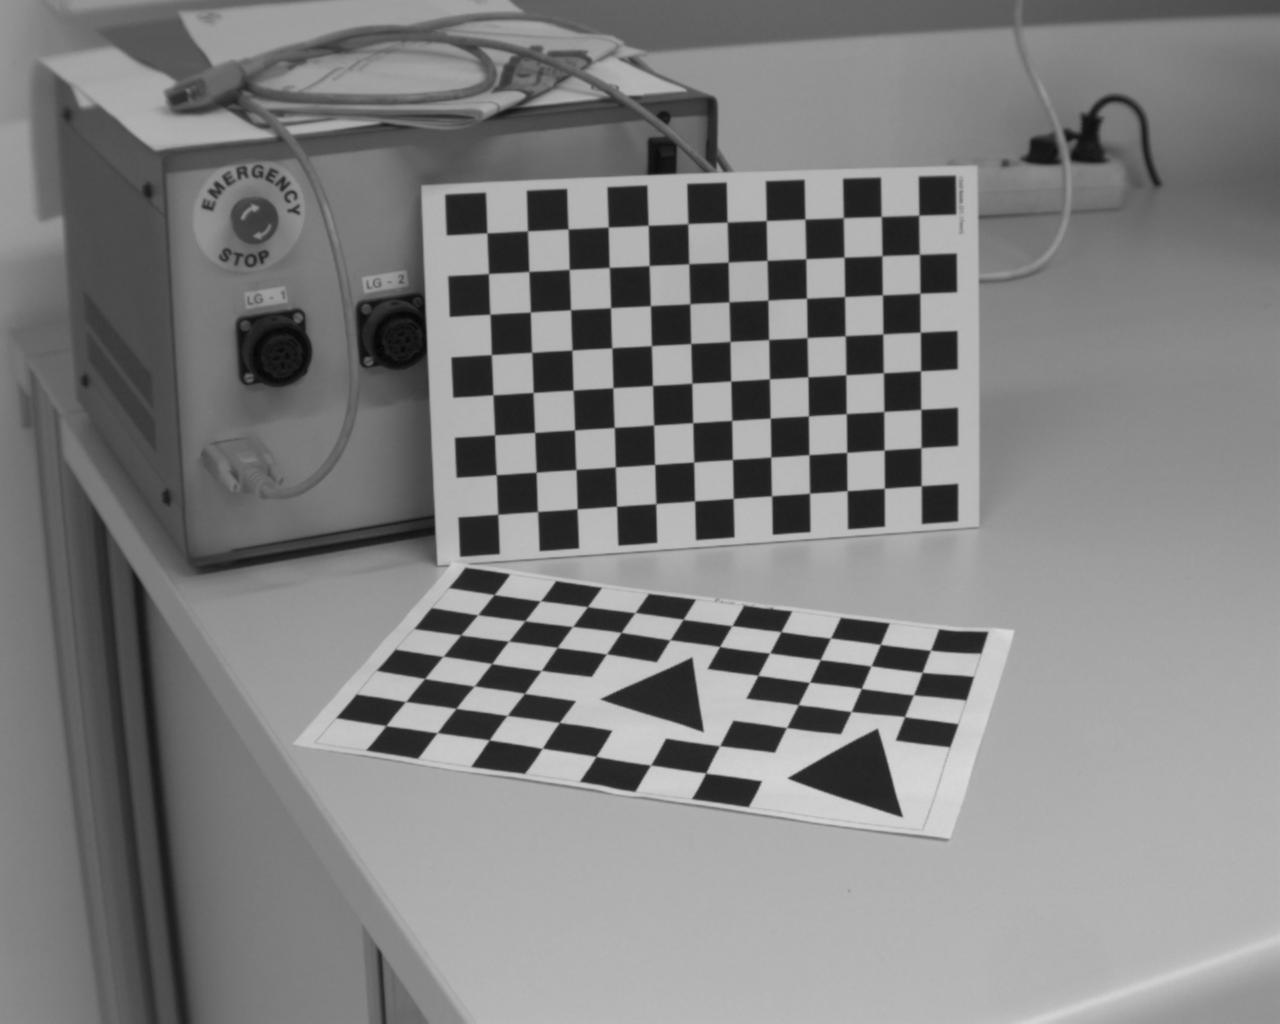
\includegraphics[scale=0.15]{Bildg_Messtechnik_Lab/FundamentalMatrix/img_left.jpg}
  \caption{Scene shot taken from left angle}
  \label{fig:sub1}
\end{subfigure}%
\begin{subfigure}{.5\textwidth}
  \centering
  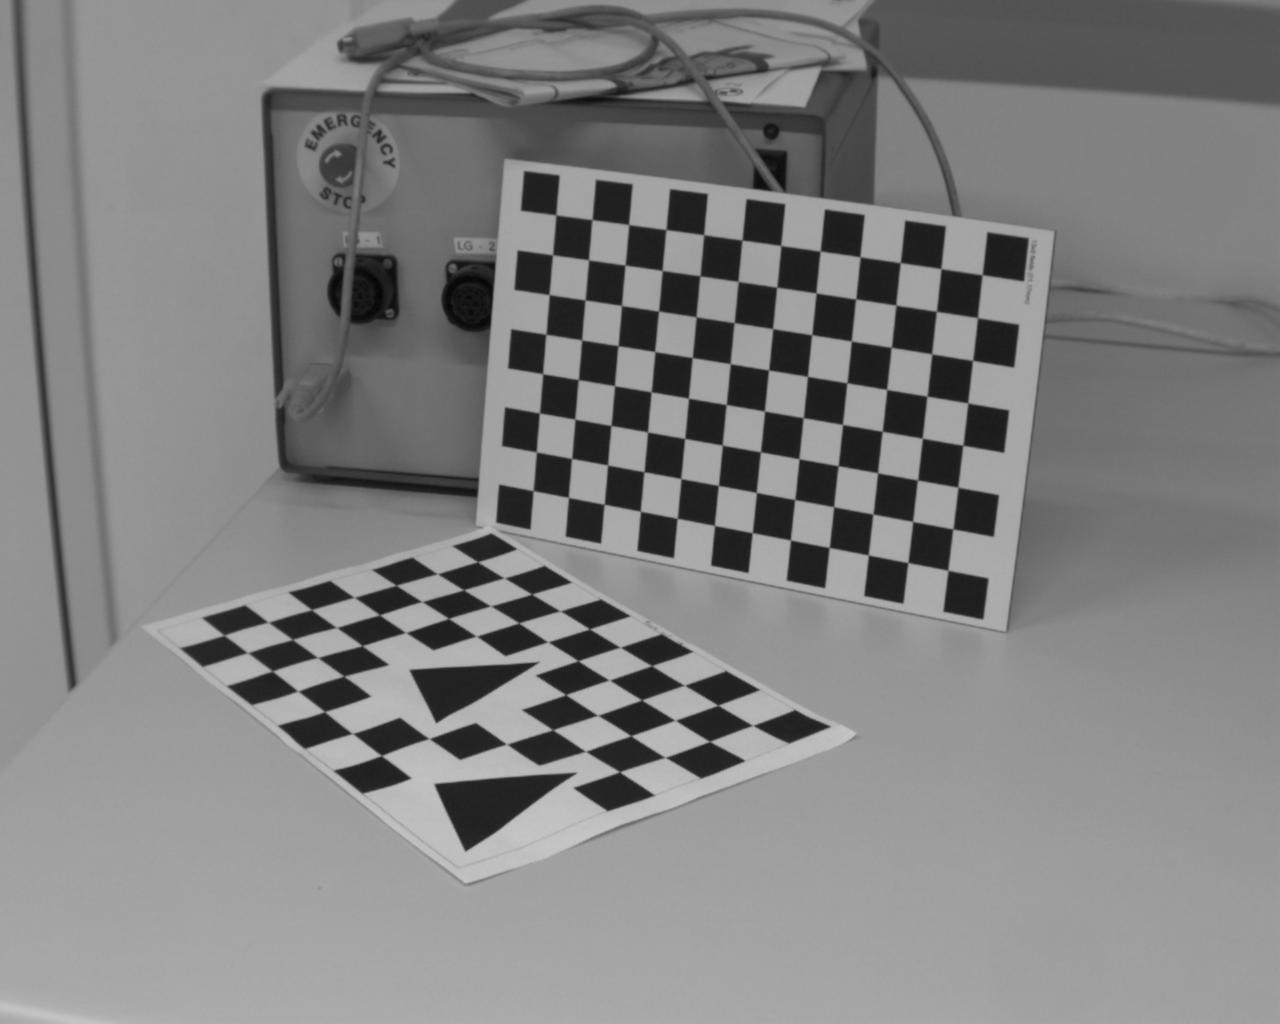
\includegraphics[scale=0.15]{Bildg_Messtechnik_Lab/FundamentalMatrix/img_right.jpg}
  \caption{Scene shot taken from right angle}
  \label{fig:sub2}
\end{subfigure}
\caption{A figure with two subfigures}
\label{fig:acquired_images}
\end{figure}


\subsubsection{Setup linear equation system}

The matrix $\mathbf{A^T}$ is calculated by multiplying all selected points in the following manner:
$$
\mathbf{A^T}_{i,j} = \left(\begin{array}{lll}
x_j' \cdot x_j \\ x_j' \cdot y_j \\ x_j' \cdot z_j\\
y_j' \cdot x_j \\ y_j' \cdot y_j \\ y_j' \cdot z_j\\
z_j' \cdot x_j \\ z_j' \cdot y_j \\ z_j' \cdot z_j\\
\end{array}\right)
$$

for $j \in [1,8]$. Then we calculate the eigenvector using the matlab function \lstinline{svd()}.
Then we only need to reshape the vector $\mathbf{f}$ to the $3$ by $3$ Fundamental matrix $\mathbf{F}$.

\begin{lstlisting}[label=lst:setup, caption=Matlab script setting up linear equation system]
A = [pts2_hom(1,:) .* pts1_hom(1,:); pts2_hom(1,:) .* pts1_hom(2,:); pts2_hom(1,:) .* pts1_hom
pts2_hom(2,:) .* pts1_hom(1,:); pts2_hom(2,:) .* pts1_hom(2,:); pts2_hom(2,:) .* pts1_hom
pts2_hom(3,:) .* pts1_hom(1,:); pts2_hom(3,:) .* pts1_hom(2,:); pts2_hom(3,:) .* pts1_hom
A = A';
[~,~,V] = svd(A);
F = reshape(V(:,end),3,3)';
\end{lstlisting}

\subsubsection{Impose rank 2 constraint}

The rank 2 constraint ($\textmd{det} \mathbf{F} = 0$) is calculated by first computing the \lstinline{svd()} of the estimated fundamental matrix $\mathbf{F}$.
This results in $\mathbf{USV^T}$. Assuming $\mathbf{S} = diag(\sigma_1, \sigma_2, \sigma_3)$ is a diagonal matrix with the singular values of $\mathbf{F}$ a new matrix
$\mathbf{\hat{F}}$ is introduced which is calculated as $Fs$ within Listing \ref{lst:constraint}.
$\mathbf{\hat{S}}$ is calculated as $diag(\sigma_1, \sigma_2, 0)$. $\mathbf{\hat{F}} = \mathbf{U\hat{S}V}$.

\begin{lstlisting}[label=lst:constraint, caption=Matlab script for imposing rank 2 constraint]
[U,S,V] = svd(F);
sig = sort(S(:),'descend');
Ss = diag([sig(1:2)' 0]);
Fs = U*Ss*V';
if USE_NORMALIZED_ALGO
Fs = T2'*Fs*T1;
end
\end{lstlisting}

\subsubsection{Show stereo pair and plot the epipolar lines}

The lines for each corresponding point are then calculated using the following equations:

$$ l' = F x $$
$$ l^T x = 0 \leftarrow y = \frac{-l_3 - l_1 \cdot x}{l_2} $$

And plotted using the \lstinline{drawEpipolarLine()} function.

\begin{figure}
 \centering
 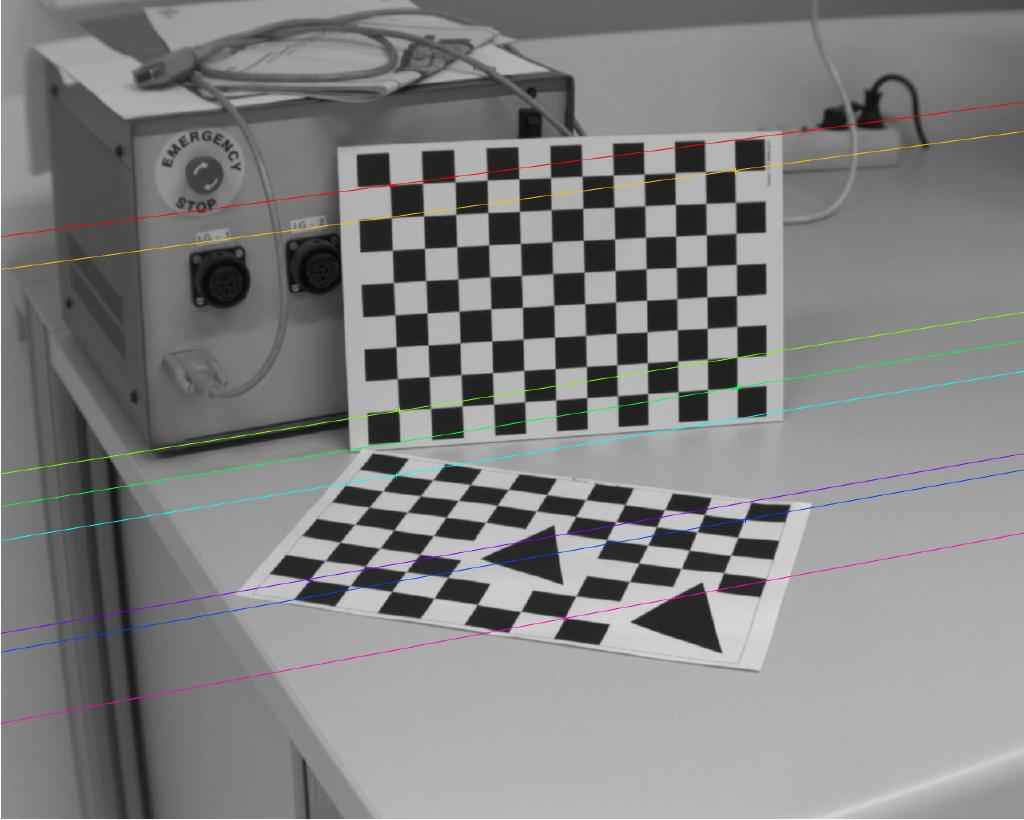
\includegraphics[scale=0.4]{left_lines.jpg}
 \caption{Epipolar lines for left Picture}
 \label{fig:left_lines}
\end{figure}


\begin{figure}
 \centering
 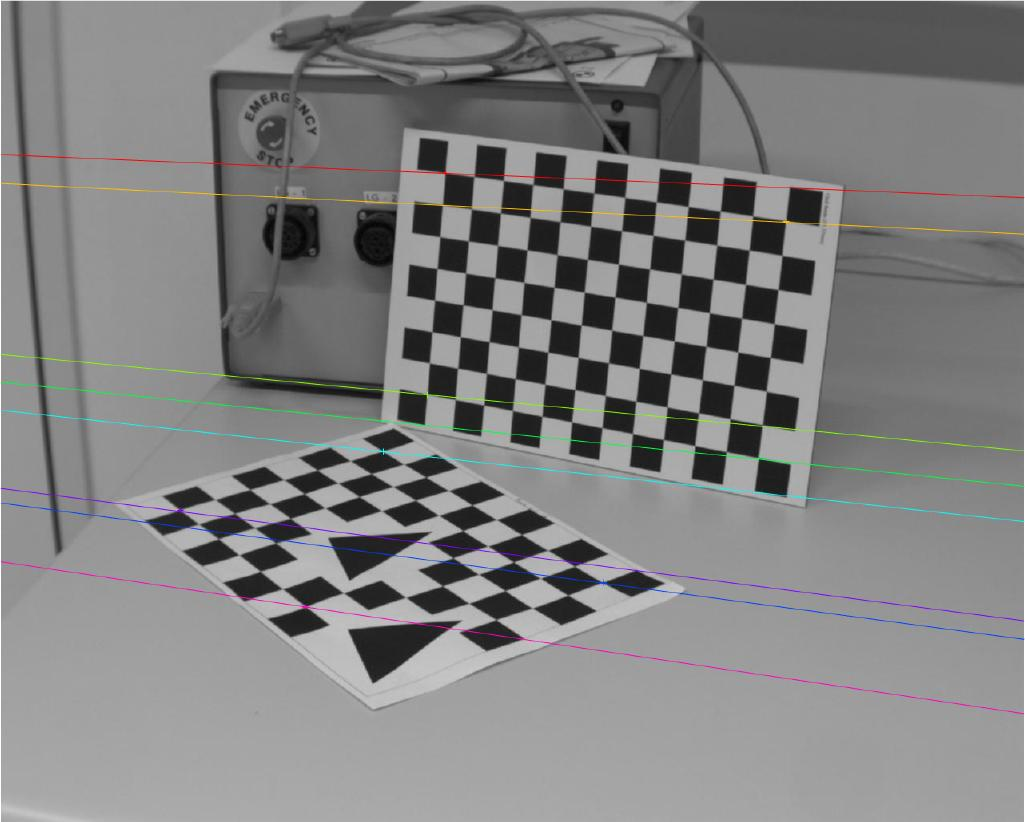
\includegraphics[scale=0.4]{right_lines.jpg}
 \caption{Epipolar lines for right Picture}
 \label{fig:right_lines}
\end{figure}


\section{Camera Projection Matrix}

\subsection{Problem statement}

Using RQ-decomposition we can decompose M = KR into K and R.
For this exercise perform the following tasks:

\begin{enumerate}
 \item Using the 3d target, acquire n = 6 images.
 \item Compute the projection matrix P using the given Matlab framework.
 \item Decompose the projection matrix P to get:
 \begin{itemize}
  \item The camera center C in the world coordinate frame.
  \item The camera calibration matrix K.
  \item The rotation matrix R that represents the orientation of the camera coordinate frame.
 \end{itemize}

\end{enumerate}

%%%
%%% end main document
%%%
%%%%%%%%%%%%%%%%%%%%%%%%%%%%%%%%%%%%%%%%%%%%%%%%%%%%%%%%%%%%%%%%%%%%%%%%%%%%%%%%

% \appendix  %% include it, if something (bibliography, index, ...) follows below

\begin{thebibliography}{XX}
  \bibitem{HO}Laboratory Handout: \textit{Lab2--Color}. \\
    Christoph Feichtenhofer and Thomas Höll, Winter--Term 2016/2017
\end{thebibliography}


%%%%%%%%%%%%%%%%%%%%%%%%%%%%%%%%%%%%%%%%%%%%%%%%%%%%%%%%%%%%%%%%%%%%%%%%%%%%%%%%
%%%
%%% bibliography
%%%
%%% available styles: abbrv, acm, alpha, apalike, ieeetr, plain, siam, unsrt
%%%
% \bibliographystyle{plain}

%%% name of the bibliography file without .bib
%%% e.g.: literatur.bib -> \bibliography{literatur}
% \bibliography{FIXXME}

\end{document}

